
\documentclass[preview,border=0.80001bp, convert=imagemagick]{standalone}
%\documentclass{article}
\usepackage{hyperref}
\usepackage{amsmath}
\usepackage{tikz}
\usepackage{miama}
\usepackage{xcolor}
\usepackage[T1]{fontenc}

\usepackage{pgfplots}

\newlength\unitlen
\tikzset{
    unit length/.code={\setlength{\unitlen}{#1}},
    unit length = 8pt
}

\begin{document}
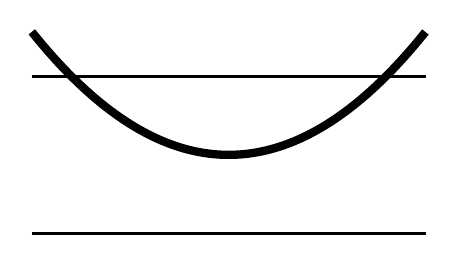
\begin{tikzpicture}[line width=3pt]
    \def\N{100}
    \def\xa{-2.5}
    \def\xb{2.5}
    \def\p{1}
    \def\h{0}
    \def\k{0}

    \draw[color=black, line width = 1pt] (\xa,-\p) -- (\xb,-\p);
    \draw[color=black, line width = 1pt] (\xa,\p) -- (\xb,\p);


    %\draw[color=black, line width = 1pt] (0,\p) -- (\xb,);

    \draw[color=black,samples=\N,domain=\xa:\xb]%
    plot(\x,{1/4*\p * (\x - \h)^2 + \k }) % r for radians
    ;

    %\draw[color=blue] (\xa,0) -- (-0.125,0);% -- (\xb,0);
    %\draw[color=blue] (0.125,0) -- (\xb,0);

\end{tikzpicture}
\end{document}
